\chapter{Estimating panel angles}
Solar panel installation angles are a large factor in deciding the energy output of a PV system. If panel angles can be freely chosen during planning and installation phases, it can make sense to either optimize for total power generation or power generation during peak consumption hours. This means that even if installation angles could be freely chosen, installation angles are unlikely to be the same for every system in the same geographical region. Panel angles may also be restricted by installation sites and mounting types. 


One reason for lacking or faulty metadata is that panel angles can be difficult to measure accurately. The tilt angle of the panels or the angle between the panel normal and zenith can easily be measured with an angle ruler and a bubble level, but the azimuth angle of the panels is much harder to measure with the same degree of accuracy. If an accurate compass is used and the difference between the magnetic north and the geographic north is taken into account, metal structures and electrical systems nearby can still distort local magnetic fields enough to cause errors in measurements. The challenges in taking accurate measurements are not insurmountable, but they may contribute to the inaccuracies and the lack of available information in PV installation parameter metadata. 

The space of possible panel installation angles can be thought as a half unit sphere in a spherical coordinate system where each point on the surface represents a direction to which the normal of the solar panels could be directed towards. A visualization of parameter space in 3D and 2D is shown in Subfigures \ref{fig_halfdome} and \ref{fig_anglespace1}. The 3 dots in the subfigure \ref{fig_anglespace1} mark the zenit for which azimuth is not well defined(red), the installation angles of FMI Helsinki installation azimuth $135^\circ$ tilt $15^\circ$(blue) and a close to power generation maximized installation with directly south facing panels with the tilt of $45^\circ$(black).


\begin{figure}[h]
	
     \centering
     \begin{subfigure}[b]{0.35\textwidth}
         \centering
         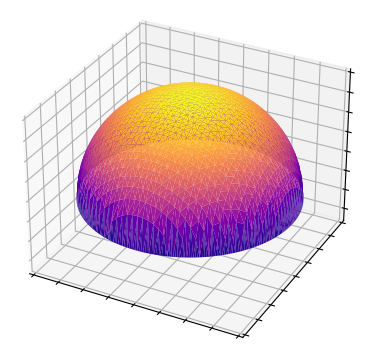
\includegraphics[width=\textwidth]{pics/halfdome}
         \caption{The space of possible angles as a 3D half sphere surface. Each point represents a possible tilt and azimuth combination.}
         \label{fig_halfdome}
     \end{subfigure}
     \hfill
     \begin{subfigure}[b]{0.35\textwidth}
         \centering
         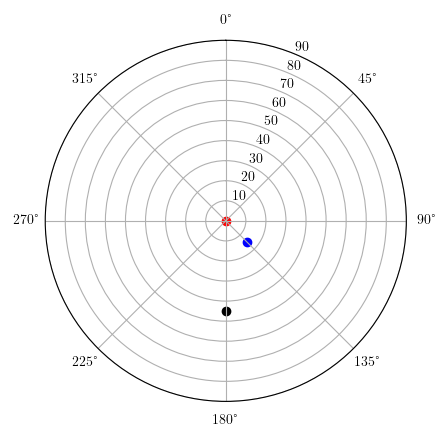
\includegraphics[width=\textwidth]{pics/polarplot}
         \caption{2D projection of the angle space, distance from center denotes the tilt angle of the panels and angle marks the azimuth.}
         
         \label{fig_anglespace1}
     \end{subfigure}
     \hfill
     \caption{Angle space visualizations.}
     \label{fig_anglespace}
\end{figure}


\noindent Estimating panel installation angles requires the use of multiple functions, each of which can be defined in multiple ways. These functions are defined in the following sections.
\begin{itemize}
  \item Prediction error function for quantifying how good a prediction was when the correct panel parameters are known.
  \item Model fitness function for measuring the difference between simulated power values and measured power values.
  %\item Multiplier matching function for matching the magnitude of simulated power values with the magnitude of measurements.
  \item Angle space discretization function for discretizing the angle space into $n$ discrete points which can then be tested with model fitness function.
\end{itemize}




\section{Prediction error function}
%The first part in developing a panel installation estimation algorithm is creating a metric for measuring how well the algorithm performs. 
In this thesis, the proposed error estimation method combines the tilt and azimuth delta values into one error angle value, the angular distance between two points on a spherical surface. The goal is then to develop a panel angle estimation function which achieves the lowest angle error value with the available datasets.

Alternative approaches can also be chosen as the function or functions for measuring the distance between two points in angle space can be defined in multiple ways. The simplest way is to use the delta of known tilt and azimuth angles as two separate error values without normalizing in any way. This method was used in Hagdadi's 2017\cite{navid_australian_article} article but such values are not direcly comparable between installations as the significance of azimuth delta depends on tilt angle.

%Measuring the distance between two coordinate pairs in angle space is more complicated than measuring errors in latitudinal or longitudinal degrees. This difficulty rises from how the azimuth angle lines converge at the pole, resulting in a coordinate system where azimuth delta values are disconnected from the phenomena which they are trying to describe. If the tilt angle is near zero, azimuth delta becomes meaningless but at high tilt angles, even small azimuth delta values can be significant. If this is not corrected for, using azimuth and tilt deltas (changes in angles) as algorithm performance metrics would incorrectly suggest that the data quality of low tilt installations is lower than that of high tilt installations, or that the system is less capable of estimating the parameters of low tilt installations. Due to these reasons, a better way of measuring the distance between two points is needed, luckily the center angle between two points on an unit sphere is easy to solve with geometry and the resulting equation is rather simple.

%While there are no issues with using angles to denote the direction of the panels, the angle values do not map the possible panel angles into the angle space in a way which would make measuring the difference between two angle space coordinates easy. The issues rises from how the azimuth angle lines converge at the pole, resulting in a coordinate system where azimuth delta values are disconnected from the phenomena which they are trying to describe. For example, a 45 degree azimuth delta is fairly significant at tilt of 90 degrees but almost insignificant at 15 degree tilt. If this is not corrected for, using azimuth and tilt deltas (changes in angles) as algorithm performance metrics would incorrectly suggest that the data quality of low tilt installations is lower than that of high tilt installations, or that the system is less capable of estimating the parameters of low tilt installations. Due to these reasons, a better way of measuring the distance between two points is needed, luckily the center angle between two points on an unit sphere is easy to solve with some geometry and the resulting equation is rather simple.

\vspace{3mm}
\noindent\textbf{Deriving angle space distance equation}

\noindent Let $v= [v_1, v_2]$ and $k = [k_1, k_2]$ be two component angle-space vectors so that $v_1$, $k_1$ $\in$ $[0,90]$ and $v_2$, $k_2$ $\in [0,360]$. These vectors represent points on the surface of a unit sphere and their components are the angles of spherical coordinate system. The cartesian coordinates of these points are:
	\begin{align}
	x_v &= sin(v_1)cos(v_2)\\
	y_v &= sin(v_1)sin(v_2)\\
	z_v &= cos(v_1)
  \end{align}
  And
  \begin{align}
	x_k &= sin(v_1)cos(v_2)\\
	y_k &= sin(v_1)sin(v_2)\\
	z_k &= cos(v_1)
  \end{align}
\noindent And the cartesian distance between these two points can be calculated with the following equation:
\begin{align}
	d = \sqrt{(x_v-x_k)^2 + (y_v-y_k)^2+(z_v-z_k)^2}
\end{align}


\noindent The two points and the origin form an isoceles triangle with the sides from the origin to the vector end points having the length of 1 while the distance between the vector end points is the same as d.

\newpage
\noindent As the lengths of three sides are known, the angles of the triangle can be calculated with the cosine rule. 
\begin{align}
	a^2 &= b^2 + c^2 - 2bc \cos(A)
\end{align}
Where
\begin{conditions}
 a     &  Side opposing the angle A, same as earlier value d \\
 b     &  Side opposing angle B, value is 1  \\   
 c	   &  Side opposing angle C, value is 1
\end{conditions}
\noindent Substituting known values into the cosine equation.

\begin{align}
	a^2 &= b^2 + c^2 - 2bc \cos(A)\\
	d^2 &= 1^2 + 1^2 - 2 \cos(A) \\
	d^2 &= 2 - 2 \cos(A)
\end{align}

\noindent Solving for angle A
\begin{align}
	d^2 &= 2-2\cos(A)\\
	2 \cos(A) &= 2 -d^2 \\
	\cos(A) &= \frac{2-d^2}{2} \\
	A &= \cos^{-1}(\frac{2-d^2}{2})
\end{align}

\noindent Renaming $A$ as $Error$.

\begin{align}
	Error &= \cos^{-1}(\frac{2-d^2}{2}) \label{errorangle}
\end{align}


\noindent By first calculating the distance between the vectors using equations 5.1-5.7 and then substituting the distance into equation 5.16, the resulting angle can then be used as an error value between two panel angle measurements. Python code based on this proof is included in appedix \ref{angular_distace_appendix}.


% This error value is the same as the angle between two points on the surface of a sphere. %In addition, if the deviation occurs only on the tilt axis, the error value and the tilt error are the same.% This makes the error values intuitive.
%In some ways, this method of calculating an error angle is analogous to moving the two angle vectors so that one of them aligns with the 0 tilt point and computing the tilt delta between the two points. Because of this, the error values are fairly intuitive and the error value should better represent the actual difference between installations than other error values calculated via other means.


\vspace{5mm}

%\section{Angle estimation error functions}
%The process of angle estimation requires the use of error estimation functions. The first function is needed for testing the accuracy of the algorithm by translating the known installation angles and the estimated angles into a meaningful error value. This is nontrivial as moving by a set angle value on the tilt and azimuth axis in spherical coordinate space result in different cartesian distances depending on the starting point. 


%The second function or set of functions is needed for evaluating how well a simulated irradiance curve fits the measurement data. Functions of this type can be used for parameter estimation by testing out possible parameter combinations and and choosing the combination which results in the lowest error between the simulated and measured values.


\newpage
\section{Simulation fitness function}
\label{section_simulation_error_function}

The earlier model delta function defined as Equation \ref{pv_model_delta} can be re-used here as the simulation fitness Equation \ref{pv_model_delta_v2}. By then computing multiple simulations with different panel angles and choosing the simulation with the best fitness, meaning lowest delta value, the panel angle values can be estimated.

\vspace{6mm}
\noindent\textbf{Simulation fitness function}
\begin{equation}
\begin{split}
\label{pv_model_delta_v2}
Delta_{model} = \sum_{t=1}^{1440} |P_{measured}(t) - P_{simulated}(t)| /1440
\end{split}
\end{equation}

\noindent As the function normalizes delta values by division with 1440, the delta for shorter days is lower than the delta for comparable long days. This should not matter for parameter estimation as the algorithm works by minimizing delta for each day independently. 

Visualization of the function is shown in Figure \ref{fig_simulation_fitness} where simulation with tilt of 90$^\circ$ and azimuth of 135$^\circ$ is tested against known power measurements from a day in FMI Helsinki dataset, resulting in an average delta of 2959.5 W delta per minute.


\begin{figure}[h]
\centering
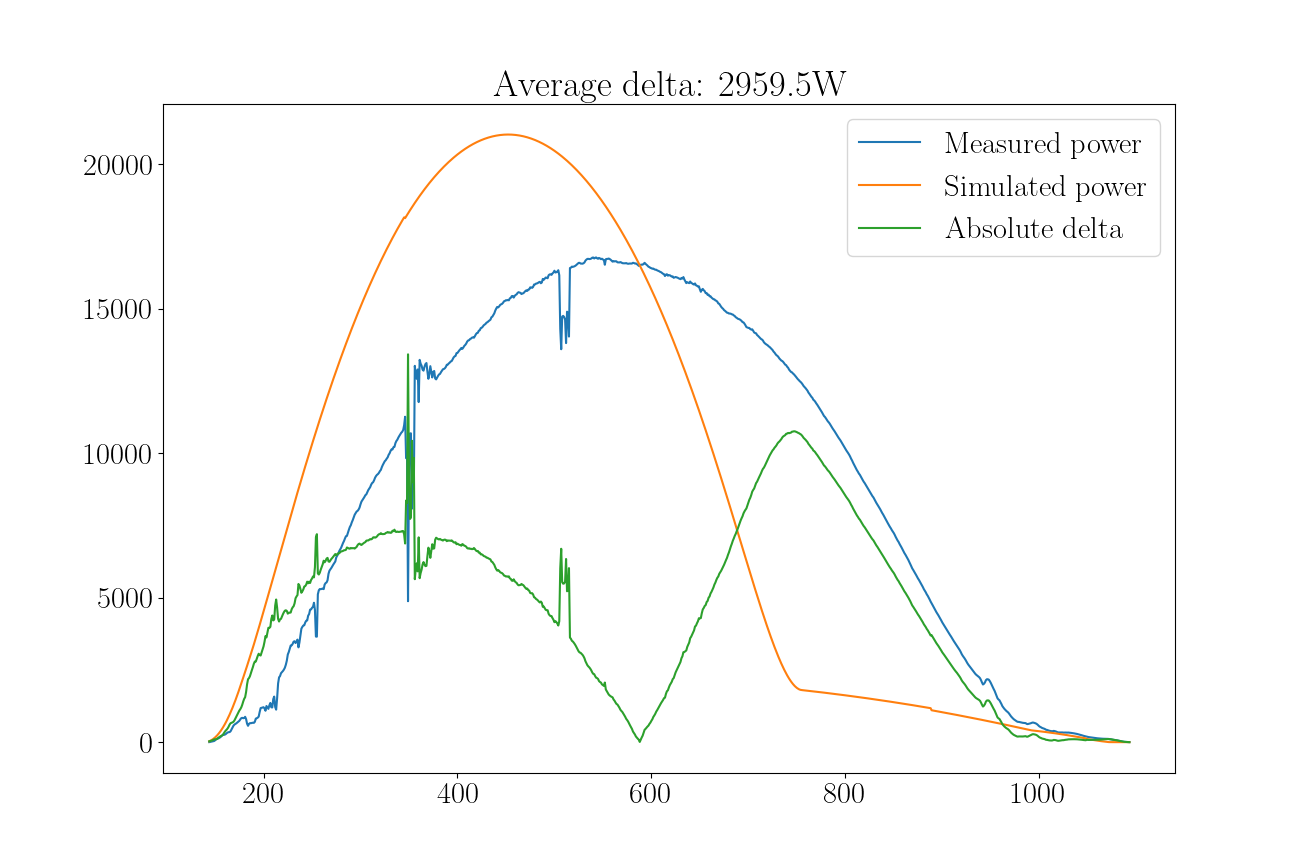
\includegraphics[width=0.85\linewidth]{pics/measured_vs_simulated} % WAS pics/measured_vs_simulated
\figcaption{Visualization of fitness function.}
\label{fig_simulation_fitness}
\end{figure}




\newpage
\section{Angle space discretization}\label{angle_space_discretization}
The next step is angle space discretization. The panel angles are denoted with a doublet of tilt and azimuth values, ranging from 0 to 90 and 0 to 360 respectively. If the tilt and azimuth axes are discretized individually in steps of 5 so that tilt is [0, 5, 10, 15... 90] and azimuth [0, 5, 10, 15... 355], the permuations of these tilt and azimuth values create an even grid in the euclidean projection of angle space where x = tilt, y = azimuth. However as the physical phenomena represented by the angle values is not a point on a flat plane but a point on a half-sphere surface, this results in an uneven discretization seen in Figure \ref{fig_5step}. 

Sphere discretization problems are relevant for 3D graphics and real world problems involving geometry and so there are pre-existing methods available for discretization. One of the mathematically more elegant methods is the Fibonacci lattice which was used in a similar fashion in González 2009 \cite{Gonzlez}. The mathematical formulation of similar lattices is an older process and an earlier example is found in Vogel 1979\cite{fibolat_old}. The following mathematical notation for the lattice is based on a code sample included in a blog post by Vagner Seibert \cite{medium_fibolat_equation}.




\noindent \textbf{Fibonacci lattice point n of k equation}
\begin{align}
	s &= n + 0.5 \\
	\phi &= acos(1 - 2 s / k) \\
	\theta &= \pi s (1 + \sqrt{5})
\end{align}
Where $n$ is the point number, $k$ is the amount of points, $\phi$ is the panel tilt angle and $\theta$ is the azimuth angle.
\begin{align}
	x &= cos(\theta)sin(\phi)\\
	y &= sin(\theta)sin(\phi)\\
	z &= cos(\phi)
\end{align}
$x$, $y$ and $z$ are the corresponding cartesian coordinates.
\vspace{5mm}


\begin{figure}
     \centering
     \begin{subfigure}[b]{0.45\textwidth}
         \centering
         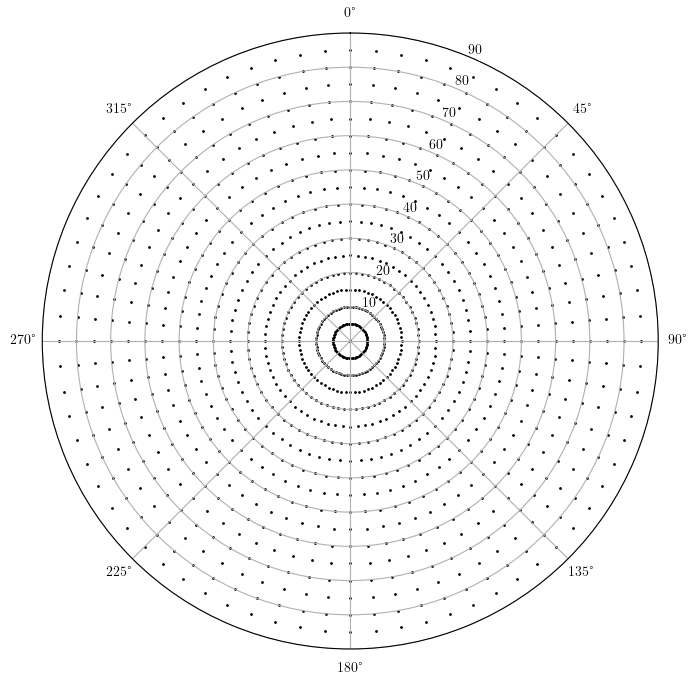
\includegraphics[width=\textwidth]{pics/disc5}
         \caption{In steps of 5 discretization with 1296 points}
         \label{fig_5step}
     \end{subfigure}
     \hfill
     \begin{subfigure}[b]{0.45\textwidth}
         \centering
         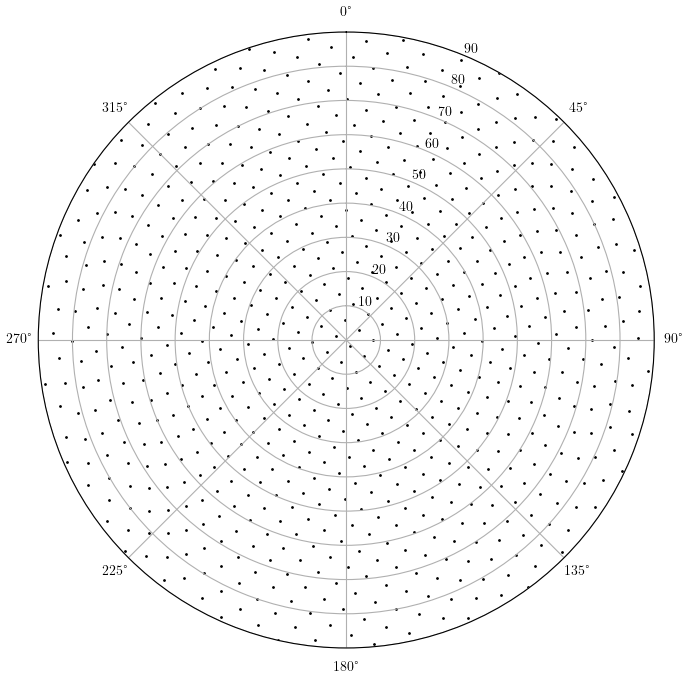
\includegraphics[width=\textwidth]{pics/fibolat1}
         \caption{Fibonacci lattice-based discretization with 756 points.}
         \label{fig_fibolat}
     \end{subfigure}
     \hfill
     
\caption{Comparison of two different discretization patterns. Fibonacci lattice based discretization on right shows a more even distribution of points than the latitude-longitude lattice. The minimum density is approximately the same in both graphs despite the difference in point counts.}
     \label{fig_5stepfibolat}
\end{figure}

\newpage
\subsection{Importance of lattice density}\label{ss_lattice_density}
Using the correct lattice density is important for using exhaustive search algorithms for panel angle estimation. Regardless of the lattice point count, a discrete lattice is unlikely to ever include the best fit in the whole $\mathbb{R}^2$ parameter subspace. This means that lattices of a sufficient density should be used in order to guarantee that a lattice point exists near to the optimal fit. However as incresing the lattice density increases the computational cost of angle estimation, choosing a good density becomes an optimization problem.

Lattice densities behave differently in different latticing patterns. With \textit{in-steps-of-n} lattices, the main benefit is easy readibility. If the lattice is given one point for latitudinal and longitudinal degree, resulting in $360*90=32400$ points, then the lattice can be aligned so that each tilt and azimuth degree pair where angles are integers is tested. This discretization makes the results easily understanble as if the known installation angles are given as integers, a point representing the exact known installation angles already exists on the lattice.

With Fibonacci lattices and other lattice patterns in which lattice points may appear to be at seemingly random coordinates, evaluation of search algorithms is more difficult without visual aid. For example, in a 1000 point Fibonacci lattice the closest point to an arbitrary angle space coordinate is not obvious nor is the center angle distance between datapoints in the lattice as intuitive as with in-steps-of lattices.


\newpage
\section{Solving panel angles}
Now that the geographic location and the multiplier values of installations are known to be solvable and fitness functions have been defined, the next step is solving the panel angles. The simple method is evaluating all points on a sufficiently dense lattice and choosing the point with the lowest delta value.

Figure \ref{fig_polar10} contains 10 Fibonacci lattice points and their normalized delta values. The best fit was at tilt 31.79$^\circ$, azimuth 153.79$^\circ$ and it had a delta value of 369W. The lattice density leaves large gaps between lattice points and this found best fit is the closest point to the known installation angles of 15$^\circ$ and 135$^\circ$. Center angle error as per Equation \ref{errorangle} is 18.17$^\circ$.




%is to solve the panel installation angles. The chosen method relies on splitting angle space into $n$ discrete points and evaluatin each of their fitness by calculating an error value. Here the angle space was split into 10 discrete points with fibonacci lattice \ref{angle_space_discretization} and the fitness of each point was evaluated with area error \ref{areaerror} and multiplier matching \ref{function_multipliermatch} functions. %The tilt-azimuth pair with the lowest error value was 31 


\begin{figure}[h]
\begin{floatrow}
\ffigbox{%
  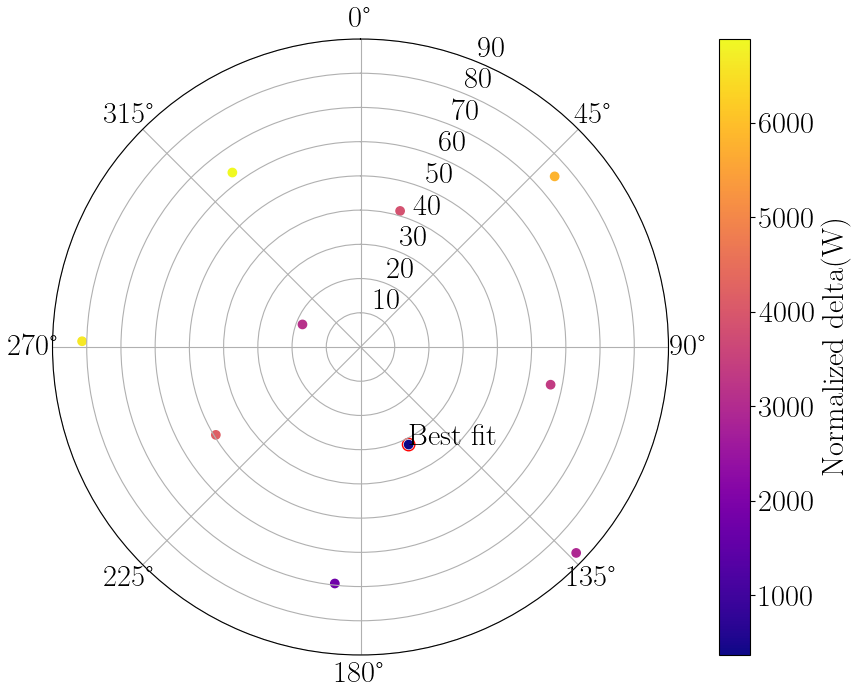
\includegraphics[width=1\linewidth]{pics/10p_fibo_fit_text} % WAS pics/10p_fibo_fit_text
}{
  \caption{Polar plot of test points for a single day of data from FMI Kumpula dataset.}
  \label{fig_polar10}
}
\capbtabbox{%
  \begin{tabular}{c|c|c} \hline

Tilt$^\circ$ & Azimuth$^\circ$ & Delta(W)\\
\hline
18.19 & 291.25 & 3128\\
\textbf{31.79} & \textbf{153.74} & \textbf{369}\\
41.41 & 16.23 & 3873\\
49.46 & 238.72 & 4183\\
56.63 & 101.22 & 3356\\
63.26 & 323.71 & 6888\\
69.51 & 186.2 & 1759\\
75.52 & 48.69 & 5814\\
81.37 & 271.18 &  6626\\
87.13 & 133.68 & 2938\\
\hline\hline
\end{tabular}
}{%
  \caption{Tilt, azimuth and error table for single day.}
}
\end{floatrow}
\end{figure}

\noindent The fit achieved with the 10 point lattice is not very good and better results can be achieved by increasing the lattice density. The trivial method is to use a Fibonacci lattice with a higher point count, for example the fit achieved with a 10 000 point lattice show in Figure \ref{10k_fits_new_helsinki} found the best fit at tilt 14.79$^\circ$, azimuth 136.2$^\circ$, delta value of 136.2W and center angle error of 0.3659 degrees$^\circ$. This is a much better fit but increasing the lattice density comes with a higher computational cost. Depending on code optimizations, evaluating a single day from the dataset against a 10 000 point lattice can take up to several hours.

\begin{figure}[h]
\centering
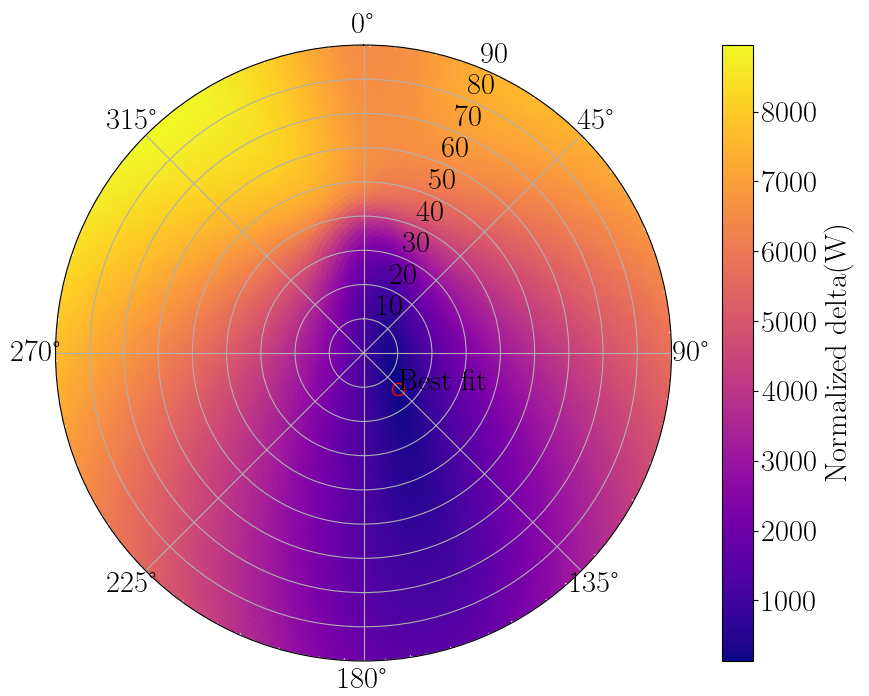
\includegraphics[width=0.8\linewidth]{pics/10k_new_model} % WAS pics/measured_vs_simulated
\figcaption{Results of a 10 000 datapoint lattice fitting against a single day from FMI Helsinki dataset. Center angle error between the found best fit and known installation angles is 0.3659$^\circ$.}
\label{10k_fits_new_helsinki}
\end{figure}



%# Best fit was tilt: 14.79 azimuth: 136.2 fitness:133.3 10k lattice result !






%\noindent Now that the method can be seen to work, it is time to improve the results. This can be done by generating larger lattices and thus by evaluating higher amount of datapoints, the algorithm has a higher chance of finding the global minimum error point. As per \ref{ss_lattice_density}, Fibonacci lattice of 1000 points would have the angular resolution of approximately 4 degrees where as 10000 points would be near to 1.5 degrees. The performance can also be improved by evaluating best fits for multiple days at once. The resulting point cloud of best fits can then be used for averaging out noise in the predictions.

%The plot \ref{fig_polar_multiyear} is a result of using the angle finding algorithm on 41 days from FMI Kumpula dataset with a Fibonacci lattice of 1000 points. The two darker spots near the center of the graph are the two most common best fits, [17.0$^\circ$, 138.4$^\circ$] with 17 and [22.7$^\circ$, 143.1$^\circ$] with 16 out of 41 days. These groupings are as close to the known installation angles of [15$^\circ$,  135$^\circ$] as could be expected from a 1000 point lattice. The next step is tightening the cluster, this can be done by adjusting the smoothness requirement of the cloud free day algorithm or by restricting the day range. In \ref{fig_polar_multiyear_summer} the tightening was accomplished with day range restrictions and 22 days were accepted by the algorithm.


%In \ref{fig_polarplot_13days} the polar plot is a result of taking the 13 best days from FMI Kumpula dataset year 2018 and using a fibonacci lattice with 500 test points. The most common best fit was [27.5$^\circ$, 150.8$^\circ$] with 5 occurances followed by [24.1$^\circ$, 138.4$^\circ$] with 4 days. These values are close to the 





%As all of the estimates converge on two neighboring points, the final step is increasing the lattice resolution further. With 10 000 point lattice, the cluster tightened further \ref{fig_polar_multiyear_helsinki10k}. Out of the 22 days, 7/22 or 32\% had best fit at [19.34, 136.87] with error of 4.38 degrees and 6/22 or 27\% at [17.74, 135.06] with error of 2.74 degrees. Rest of the best fits were distributed in smaller clusters near these points. The lowest angle distance best fit was [17.09, 130.32] with angle distance of 2.46 degrees. As the angle distance errors are higher than the discretization resolution and as the predicted angles are systematically biased, it would seem that the error is caused by the solar irradiance model or model fitting and not angle space discretization.


%As the angle distance errors are higher than the discretization resolution and as the results seem biased, the errors of the estimation algorithm would seem to be caused by inaccuracies in model fitting and not angle space discretization.




%\begin{figure}[h]
%\centering
%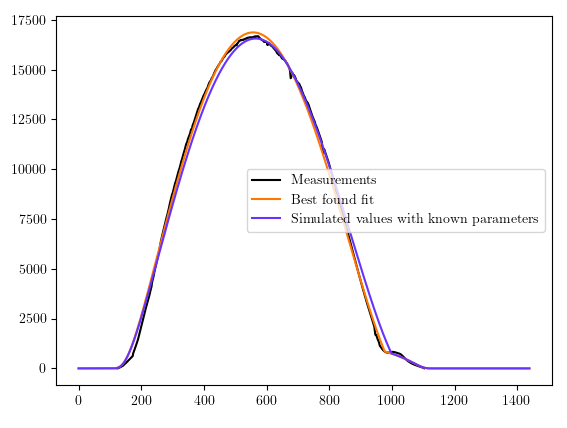
\includegraphics[width=0.8\linewidth]{pics/10kfitshelsinkiplot}
%\caption{Comparison between measured values, simulated values with known installation parameters and best found fit.}
%\label{fig_10kfitshelsinkiplot}
%\end{figure}



%day 141 predicted 17.74 135.06 delta degrees: 2.74 x
%day 145 predicted 19.92 141.6 delta degrees: 5.3
%day 148 predicted 19.34 136.87 delta degrees: 4.38 	x
%day 179 predicted 17.74 135.06 delta degrees: 2.74 x
%day 197 predicted 21.37 143.41 delta degrees: 6.87 y
%day 198 predicted 18.37 139.79 delta degrees: 3.64
%day 199 predicted 19.34 136.87 delta degrees: 4.38		x
%day 157 predicted 19.92 141.6 delta degrees: 5.3
%day 169 predicted 18.37 139.79 delta degrees: 3.64
%day 202 predicted 17.74 135.06 delta degrees: 2.74 x
%day 208 predicted 21.37 143.41 delta degrees: 6.87 y
%day 143 predicted 19.34 136.87 delta degrees: 4.38		x
%day 155 predicted 19.92 141.6 delta degrees: 5.3
%day 164 predicted 19.92 141.6 delta degrees: 5.3
%day 166 predicted 17.74 135.06 delta degrees: 2.74 x
%day 171 predicted 19.34 136.87 delta degrees: 4.38		x
%day 174 predicted 17.09 130.32 delta degrees: 2.46
%day 175 predicted 17.74 135.06 delta degrees: 2.74 x
%day 177 predicted 17.74 135.06 delta degrees: 2.74 x
%day 178 predicted 19.34 136.87 delta degrees: 4.38		x
%day 179 predicted 19.34 136.87 delta degrees: 4.38		x
%day 200 predicted 19.34 136.87 delta degrees: 4.38		x



%day 145 predicted 32.09 196.89 delta degrees: 18.65 x
%day 192 predicted 30.5 198.01 delta degrees: 16.96 y
%day 199 predicted 30.5 198.01 delta degrees: 16.96 y
%day 210 predicted 34.52 197.58 delta degrees: 20.9 z
%day 212 predicted 32.09 196.89 delta degrees: 18.65 x
%day 213 predicted 35.07 194.65 delta degrees: 21.86 k
%day 167 predicted 27.07 200.24 delta degrees: 13.37 i
%day 143 predicted 30.5 198.01 delta degrees: 16.96 y
%day 144 predicted 28.83 199.13 delta degrees: 15.21 l
%day 145 predicted 28.83 199.13 delta degrees: 15.21 l
%day 162 predicted 27.07 200.24 delta degrees: 13.37 i 
%day 167 predicted 27.07 200.24 delta degrees: 13.37 i 


\newpage
%\subsection{Performance on single day estimation with Helsinki dataset}
\noindent The results of the exhaustive search algorithm are excellent for the Helsinki dataset. Angle delta values as low as the achieved 0.37$^\circ$ are low enough to be within the assumed 1$^\circ$ precision of known installation angles. 

The next verification step is using the algorithm on multiple days from the same dataset and checking the spread pattern. This was done on sets of days with both Helsinki and Kuopio datasets. Figures \ref{fig_fmi_helsinki_1000_multi_day_2018} and \ref{fig_fmi_helsinki_1000_multi_day_2020} display the tight scatter patterns in the Helsinki predictions. For the tight grouping in the 2018 figure the average tilt of 13.89$^\circ$ and azimuth of 130.81$^\circ$ are close reported angles of 15$^\circ$ tilt and 135$^\circ$ azimuth. And with year 2019 where the scatter pattern is wider, the average of the results is 14.17$^\circ$ tilt, 132.62$^\circ$ azimuth which are both even closer to the known installation angles. Fitness values or the per minute delta values are for the multi day 10 000 point evaluations were in the range of 76W to 117W for the Helsinki dataset.

%years such as 2019 where the scatter pattern is wider, the average of the results

%and center angle delta of X$^\circ$ 

% Average tilt:13.4 azimuth:128.06 fitness111 helsinki 2017
% Average tilt:13.89 azimuth:130.81 fitness84 Helsinki 2018
% Average tilt:14.17 azimuth:132.62 fitness117 Helsinki 2019
% Average tilt:13.54 azimuth:128.78 fitness76 Helsinki 2020
% Average tilt:15.04 azimuth:134.25 fitness90 Helsinki 2021
% The tight clustering visible in both figures suggest that the  



%By using the same method and plotting the best fits for several cloud free days from one dataset, the found best fits cluster tightly around the known installation angles as seen in figures \ref{fig_fmi_helsinki_1000_multi_day_2018} and \ref{fig_fmi_helsinki_1000_multi_day_2020}. The years 2018 and 2020 were chosen for higher number of days passing the set cloud free day selection threshold.


\begin{figure}[!h]
\begin{floatrow}
\ffigbox{%
  	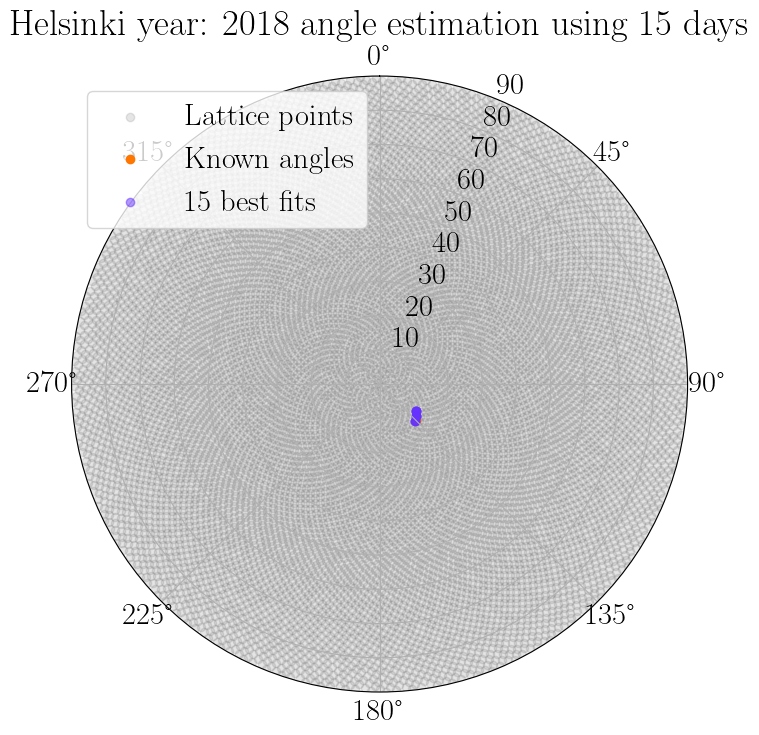
\includegraphics[width=1\linewidth]{pics/Helsinki2018}
}{
  	\caption{10 000 point exhaustive search on 15 cloud free days from FMI Helsinki dataset using year 2018.}
  	\label{fig_fmi_helsinki_1000_multi_day_2018}
}	

\ffigbox{%
  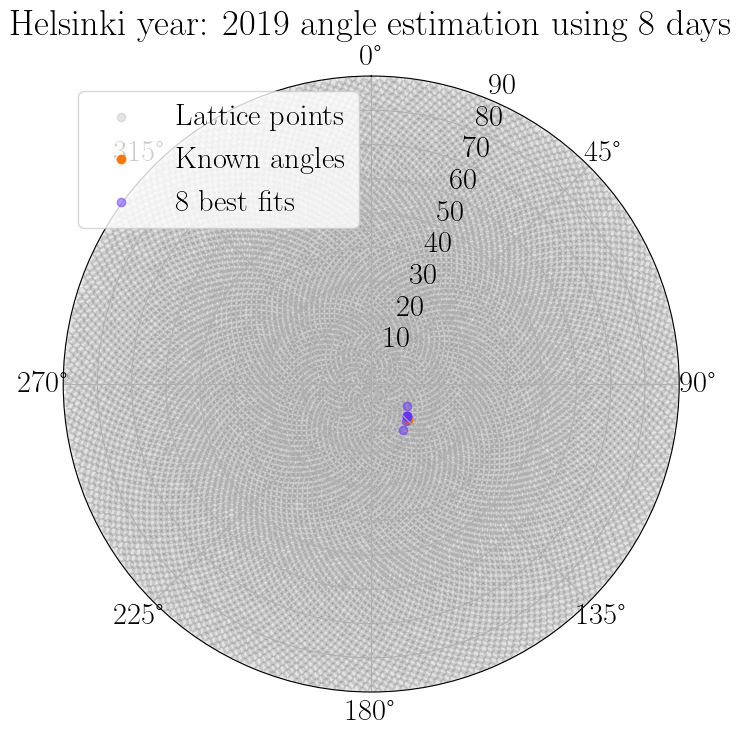
\includegraphics[width=1\linewidth]{pics/Helsinki2019}
}{
  \caption{10 000 point exhaustive search on 8 cloud free days from FMI Helsinki dataset using year 2019.}
  \label{fig_fmi_helsinki_1000_multi_day_2020}
}
\end{floatrow}
\end{figure}

\noindent Results for the Kuopio dataset are not nearly as good as the Helsinki predictions. Figures \ref{fig_fmi_kuopio_10000_multi_day_2018} and \ref{fig_fmi_kuopio_10000_multi_day_2020} clearly indicate that estimations are converging approximately 13 degrees off from the known installation angles. The reason for this significant delta is not known and there could be multiple contributing factors. One possible explanation is panel shading which is more likely to occur when the Sun is near the horizon. This causes a proportionally higher energy output loss during first and last hours of the day, resulting in a more narrow power generation plot shape. This \textit{sharpness} is also influced by the tilt angle of an installation as was previously seen in Figure \ref{fig_poa_different_parameters} and thus the error in the estimated tilt angle could be partially caused by either panel self shadowing or shadowing caused by other stuctures near the PV panels.

%Similar patterns occur with all of the years from FMI Helsinki and Kuopio datasets where estimated angles form clusters in angle-space. With Helsinki the delta between known installation angles and estimations is minimal where as with the Kuopio dataset the cluster is larger and offset by a bias of approximately 13$^\circ$.


%average delta angle: 12.956
%Average tilt:26.76 azimuth:201.11 fitness290

\begin{figure}[h]
\begin{floatrow}
\ffigbox{%
  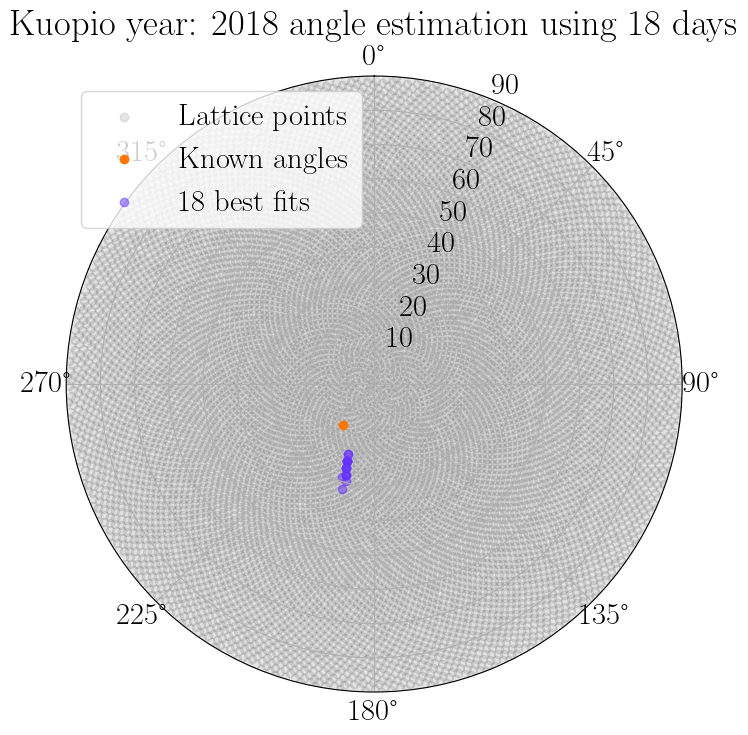
\includegraphics[width=1\linewidth]{pics/Kuopio2018} % WAS pics/10p_fibo_fit_text
}{
  \caption{10 000 point exhaustive search on 18 cloud free days from FMI Kuopio dataset using year 2018.}
  \label{fig_fmi_kuopio_10000_multi_day_2018}
}

\ffigbox{%
  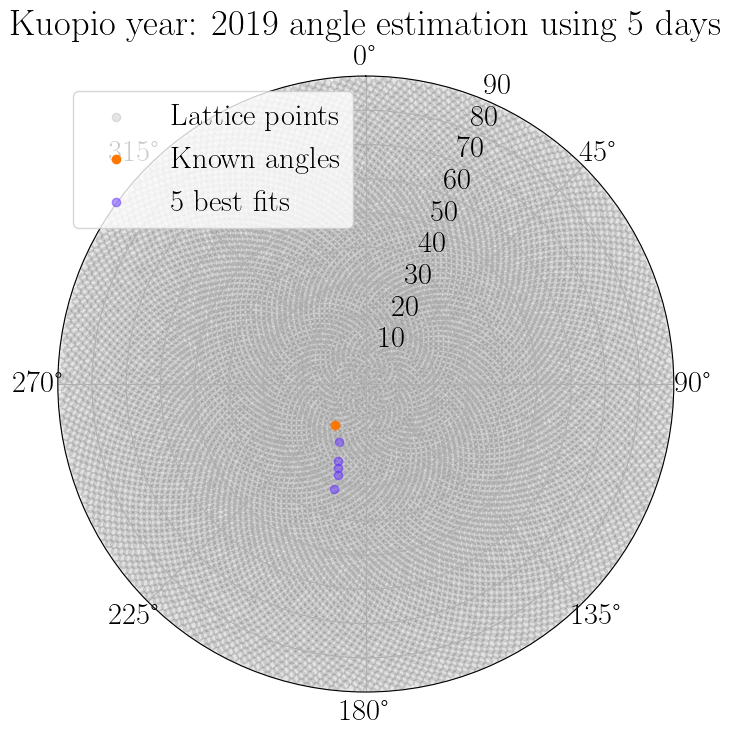
\includegraphics[width=1\linewidth]{pics/Kuopio2019} % WAS pics/10p_fibo_fit_text
}{
  \caption{10 000 point exhaustive search on 10 cloud free days from FMI Kuopio dataset using year 2020.}
  \label{fig_fmi_kuopio_10000_multi_day_2020}
}
\end{floatrow}
\end{figure}


\newpage

\clearpage

\section{Solving panel angles iteratively}
The exhaustive search used in earlier section suggest that the method is capable of estimating panel installation angles accurately. However evaluating 10 000 point lattices is somewhat inelegant and this can be avoided by using multiple less dense lattices iterarively if the fitness space satisfies some requirements.

The first requirement is that the fitness space should be smooth. This smoothness does not have to be perfect, fine patterns and details in the fitness space surface do not cause issues with iterative search algorithms if the noise pattern is not observable in the iterative lattices. Based on an earlier Figure \ref{10k_fits_new_helsinki} generated by exhaustive search, this requirement would appear to be met.

Second requirement is that the fitness space should contain as few convergence points and their respective basins as possible. These basins are regions in fitness space which are defined by a convergence point and their surrounding regions where the slope of the space leads to the respective convergence point. The region around best found fit in Figure \ref{10k_fits_new_helsinki} forms a large basin but there would also appear to be a second converge point somewhere around azimuth 0$^\circ$ tilt 90$^\circ$.

 

\noindent \textbf{Iterative panel angle estimation algorithm}
\begin{enumerate}
	\item Choose a cloud free day from the dataset for evaluation.
  \item Choose a starting or "center" point from the angle space. This can be either the best result from a low density lattice or a fixed point such as tilt 45$^\circ$ azimuth 180$^\circ$.
  \item Evaluate the fitness at the center point and store that as the center point fitness.
  \item Choose a few points near this center point within a given distance and evaluate their fitness. If any of the neighboring points results in a better fit than the center point, this point will then be chosen as the new center point.
  \item Repeat steps 3 and 4 until step 4 does not find a better fit. When this happens, decrease the distance used for the local lattice in step 4.
  \item Repeat steps 3,4 and 5 for a set number of times. Last center point is the best iteratively found fit.
\end{enumerate}


\begin{figure}[H]
     \centering
     \begin{subfigure}[b]{0.45\textwidth}
         \centering
         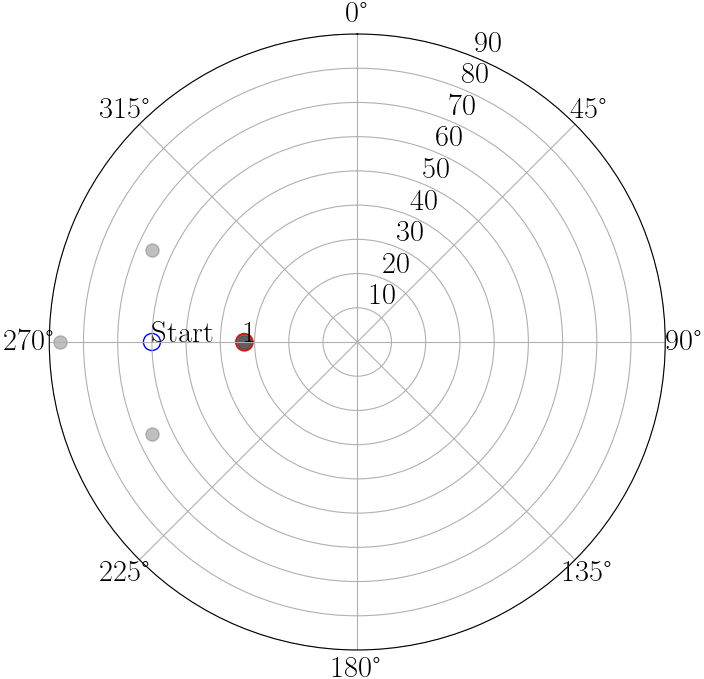
\includegraphics[width=\textwidth]{pics/iterative_1_step}
         \caption{Iterative best fit search after 1 cross pattern search.}
         \label{fig_iterative_1_step}
     \end{subfigure}
     \hfill
     \begin{subfigure}[b]{0.45\textwidth}
         \centering
         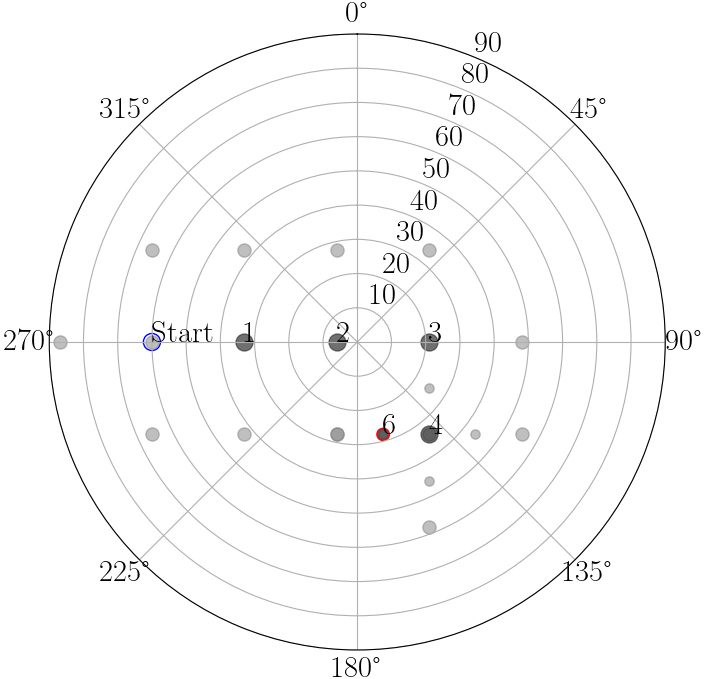
\includegraphics[width=\textwidth]{pics/iterative_6_step}
         \caption{Iterative best fit search after 6 cross pattern searches.}
         \label{fig_iterative_6_step}
     \end{subfigure}
     \hfill
     
     
\caption{Visualization of a + pattern iterative best fit search algorithm. Numbers next to markers indicate that a point was the best found during n:th cross pattern search.
% Starting point was chosen to be tilt 60$^\circ$ azimuth 270$^\circ$ for visualization reasons.%Number 5 is missing from \ref{fig_iterative_6_step} as no new best fit was found, resulting in search distance deacrease. Red circle marks the best found fit.
}
     \label{fig_iterative_visual_1}
\end{figure}

\newpage

\subsection{Local lattice generation}
The step 4 in the iterative panel angle solving algorithm detailed above is the first non-trivial step in the algorithm as it requires the generation of local lattices. One option would be to use a subsection of a Fibonnaci lattice, but generating large Fibonnacci lattices and utilizing only a small subsection would require unnecessary computation. 

The method shown in Subfigure \ref{fig_iterative_1_step} is based on generating a + pattern by first transferring the starting point from angle space to a unit disk with Equation \ref{angle_space_to_unit_circle}. On this unit disk 4 points are generated, each of which is $s$ units away from the start point either on x or y -axis using pattern from Equation \ref{local_lattice_from_xy}. When these 4 points are transformed back into angle space with \ref{unit_circle_to_angle_space}, they can be used as the local lattice surrounding the chosen center point.

\noindent \textbf{Angle space to unit disk equations}
\begin{equation}
\begin{split}
\label{angle_space_to_unit_circle}
d &= Tilt/90^\circ \\
x &= cos(Azimuth)d \\
y &= sin(Azimuth)d \\
\end{split}
\end{equation}


\noindent \textbf{Unit disk points}
\begin{equation}
\begin{split}
\label{local_lattice_from_xy}
p_1 &= (x+s,y) \\
p_2 &= (x-s,y) \\
p_3 &= (x,y+s) \\
p_4 &= (x,y-s) \\
\end{split}
\end{equation}

\noindent \textbf{Unit disk to angle space equations}

\begin{equation}
\begin{split}
\label{unit_circle_to_angle_space}
d &= x^2+y^2\\
Tilt &= \sqrt{d}*90^\circ\\
Azimuth &= tan^{-1}2(x/d, y/d)
\end{split}
\end{equation}

\pagebreak

\subsection{Results}
By using 30 iterations with initial search distance of 0.3 on a set of cloud free days from the FMI Helsinki and Kuopio dataset, scatter patterns shown in Figures \ref{iterative_multiday_helsinki2019} and \ref{iterative_multiday_kuopio2019} are generated. The center angle distances between known angles and cluster means for the Helsinki and Kuopio scatter patterns are 1.97$^\circ$ and 12.47$^\circ$ respectively. The Helsinki scatter pattern is marginally worse than the pattern achieved by exhaustive search algorithm were as results for Kuopio data seem to have a similar large bias as before with the exhaustive algorithm. Exact values vary depending on day smoothness requirements and chosen year.

%Average tilt: 14.404 azimuth: 132.361
%Fitness: 114.9164
%Cluster CAD: 0.897

\begin{figure}[H]
     \centering
     \begin{subfigure}[b]{0.45\textwidth}
         \centering
         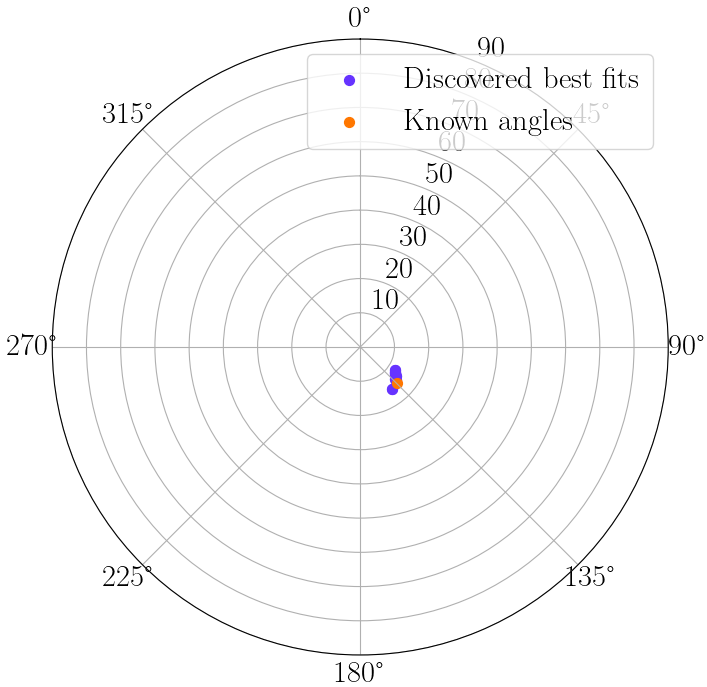
\includegraphics[width=\textwidth]{pics/iterative_multiday_helsinki}
         \caption{Iterative search used on 8 days from FMI Helsinki dataset.}
         \label{iterative_multiday_helsinki2019}
     \end{subfigure}
     \hfill
     \begin{subfigure}[b]{0.45\textwidth}
         \centering
         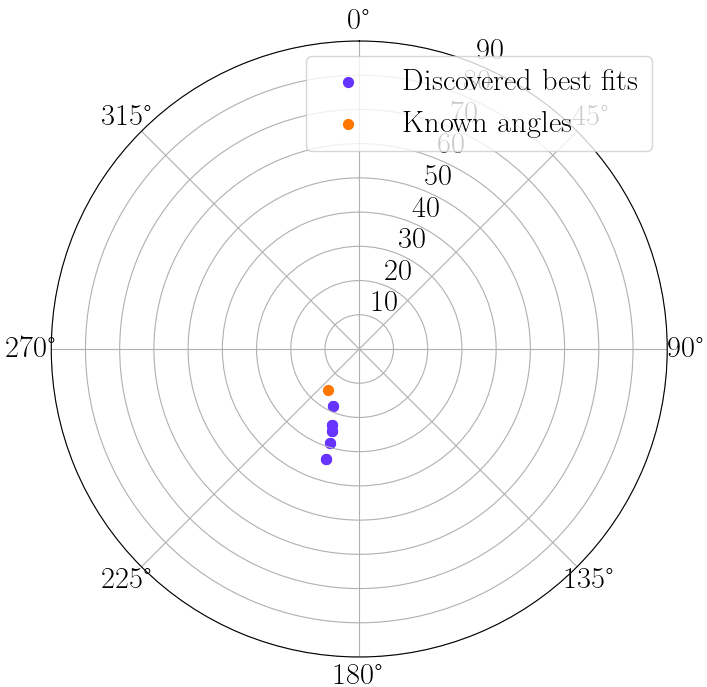
\includegraphics[width=\textwidth]{pics/iterative_multiday_kuopio}
         \caption{Iterative search used on 5 days from FMI Kuopio dataset.}
         \label{iterative_multiday_kuopio2019}
     \end{subfigure}
     \hfill
     
     
\caption{Scatter patterns for iterative panel estimation algorithm on multiple days.}

%Cluster parameters: KUOPIO
%Average tilt: 25.98 azimuth: 199.437
%Cluster CAD: 12.47

%Cluster parameters:
%Average tilt: 13.385 azimuth: 130.392
%Cluster CAD: 1.97

%Cluster parameters: Helsinki 2020
%Average tilt: 13.697 azimuth: 129.645
%Fitness: 86.5242
%luster CAD: 1.859

     \label{fig_iterative_visual_1}
\end{figure}

\noindent One method for comparing the iterative method against the exhaustive is to compare the fitness values achieved by both methods. If for example the resulting fitness values are better for the exhaustive search, then there could be multiple convergence points in the basin of the fitness space and the iterative function could be converging on the wrong point. Where as if the iterative method achieves worse center angle distances and better fitness values than the exhaustive, the seemingly worse results of the iterative method would be a result of a better fit existing in the angle space which the Fibonnacci lattice points did not contain. 

By testing out individual days and sets of days, the difference between achieved fitness values with the different estimation methods do not seem to vary significantly. For the Helsinki dataset the fitness values are somewhere in the 75W to 120W range for both algorithms depending on chosen parameters, with even performance with both algorithms. This is also visible in Figures \ref{measured_vs_simulated_vs_estimated} and \ref{measured_vs_simulated_vs_estimated_kuopio} where the curves generated by the results of both search methods are indistinguishable.

%By using the year 2020 from the Helsinki dataset, filtering cloud free days with threshold of 1.5\% and accepting days 22 from day range of 120 to 250, the resulting fitness is 86W and center angle delta of 0.6$^\circ$. This means that the best found fit had an approximate deviation of 86W per minute. For the exhaustive search algorithm these fitness values were in the range of 76W to 117W.


\subsection{Choosing between exhaustive and iterative angle estimation methods}
Both methods are capable of achieving good to results depending on data quality and algorithm parameters. As there are multiple algorithm parameters and as the exhaustive is computationally expensive, it is difficult to prove that one method is more accurate than the other. Each day in the datasets has an unique fitness space and parameters such as initial search distance, starting point and lattice point counts have a small and difficult to measure effects on the results of the algorithms.

That being stated, the computational speed of the iterative method is much higher than that of exhaustive search algorithms. If 30 steps are used with a 4 point local lattice, estimating the panel angles for a single day require 121 simulations and comparisons. This means that approximately 83 days can be iteratively evaluated in the time it takes to exhaustively evaluate one day with a 10 000 point lattice. As the 30 step iterative search algorithm reaches search distances as low as $9e-6$ units on the unit disk, the iterative method is using finer precision than would practical and the speed of the iterative algorithm can be increased further by setting a search distance limit.

Instead of choosing one method, the two search methods can be combined and used together. An iterative method with 5 to 10 steps is enough to find the general location of the best fit and a local subsection of a dense Fibonnaci lattice could be used in order to search a subsection of the angle space. This would however increase the algorithm complexity for small potential gains.

Figure \ref{measured_vs_simulated_vs_estimated} shows a comparison of fitting results for a single day. There the difference between pover curves is not significant regardless of the estimation method used and thus iterative method may be preferable. The difference between exhaustive and iterative search is likewise imperceivable in the example from FMI Kuopio dataset seen in Figure \ref{measured_vs_simulated_vs_estimated_kuopio} despite the higher center angle distance achieved with both exhaustive and iterative methods in all earlier examples.


\begin{figure}[!h]
\centering
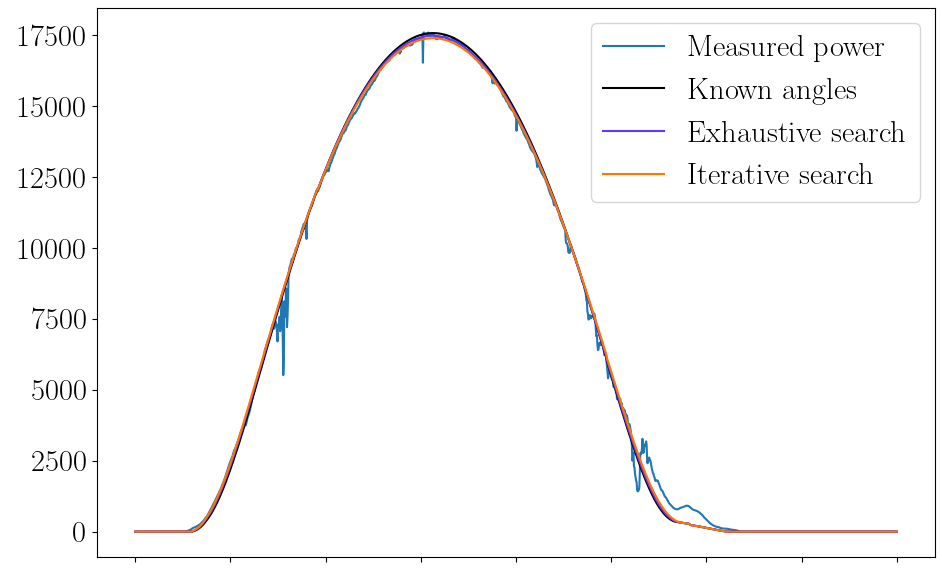
\includegraphics[width=0.8\linewidth]{pics/measured_vs_simulated_vs_estimated}
\figcaption{Comparison of power curves from measurements, simulation with known installation angles and estimated panel angles with exhaustive and iterative method. Using day 150 from year 2019 in Helsinki dataset.}
\label{measured_vs_simulated_vs_estimated}
\end{figure}

\begin{figure}[!h]
\centering
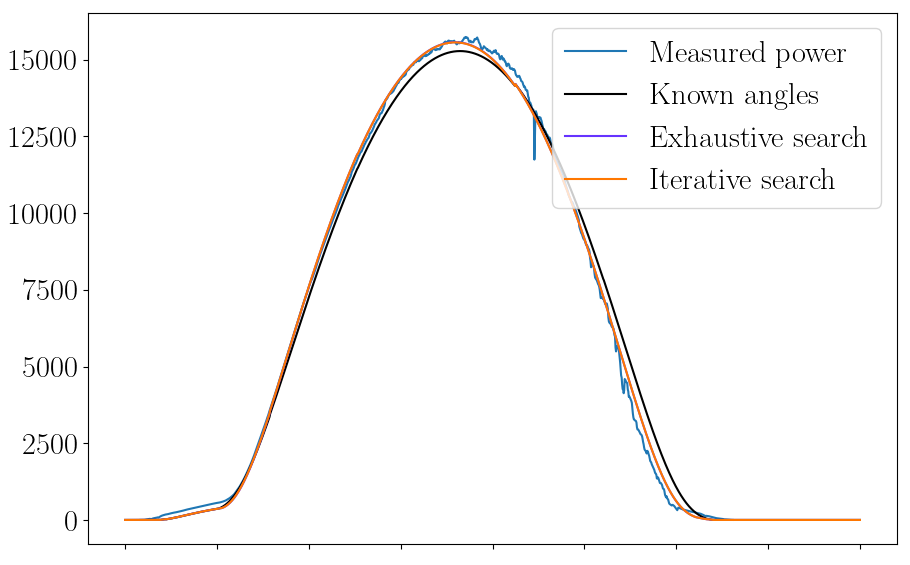
\includegraphics[width=0.8\linewidth]{pics/measured_vs_simulated_vs_kuopio}
\figcaption{Comparison of power curves from measurements, simulation with known installation angles and estimated panel angles with exhaustive and iterative method. Using day 167 from year 2019 in Kuopio dataset.}
\label{measured_vs_simulated_vs_estimated_kuopio}
\end{figure}

\pagebreak
\pagebreak

\subsection{Further development ideas}
Both algorithms perform well enough to make some of the assumptions made on the properties of fitness spaces practically irrelevant. Thus concepts of basins were not explored thoroughly but they and the field of dynamic systems which studies attractors and basins could offer additional insights into similar optimization problems.

The problem of model fitting for angle estimation may also have connections to convolutions. Understanding the mathematical properties of signal impulses and their convolution shapes could help in proving how likely the formation of multiple basins are. This could be beneficial in starting point selection with iterative fitting algorithms.

The estimation algorithms should be evaluated with multiple different datasets in order to determine whether results from the Kuopio data are an anomaly or the algorithms are as noise sensitive as the Kuopio data suggests. Similarly data from different sources and with different temporal resolutions would help in verifying how well the algorithms perform with available data.








